\chapter*{Preface}
\addcontentsline{toc}{chapter}{Preface}
Theses at the faculty of mathematics and physics usually fit into one of three categories:
\begin{enumerate}
\item Theoretical thesis
\item Experimental thesis
\item Implementation thesis
\end{enumerate}
My thesis does not fit entirely into only one category and it does not try to. The project consists of several similarly important parts which are:
\begin{itemize}
\item Design of the algorithm for generating a special binary matrix
\item Making it run fast on inputs which are usual for researchers
\item Implementing the algorithm to provide practical tool
\end{itemize}
None of these points would make sense alone but together the thesis may become very useful for scientists as it is provides with a process generating random matrices and it is a common practice to test hypothesis on random data.
\chapter*{Introduction}
We denote by $M\in\{0,1\}^{n\times m}$ a \emph{binary matrix} of size $n$ by $m$, calling $n$ the number of rows of $M$ - the \emph{height} of the matrix $M$ and $m$ the number of columns - its \emph{width}. A \emph{line} of a matrix is one of its rows or columns and we denote by $L(M)$ the ordered set of all lines of $M$. Its order is given by the natural indexing of rows and columns.

\begin{defn}
We say a binary matrix $M$ \emph{contains} a binary matrix $P$, which we call a ``pattern'', as a submatrix, if there is a mapping $f:L(P)\rightarrow L(M)$, such that
\begin{itemize}
\item $l\in L(P)$ is a row of $P$ iff $f(l)\in L(M)$ is a row of $M$
\item $\forall l,l'\in L(P):$ $l<l'\Rightarrow f(l)<f(l')$ (preserves the order)
\item $\forall l,l'\in L(P):$ if lines $l$ and $l'$ intersect and there is a one-entry at the intersection, then there is a one-entry at the intersection of $f(l)$ and $f(l')$.
\end{itemize}
otherwise, it \emph{avoids} the pattern $P$.
\end{defn}
\begin{figure}[h!]
\centering
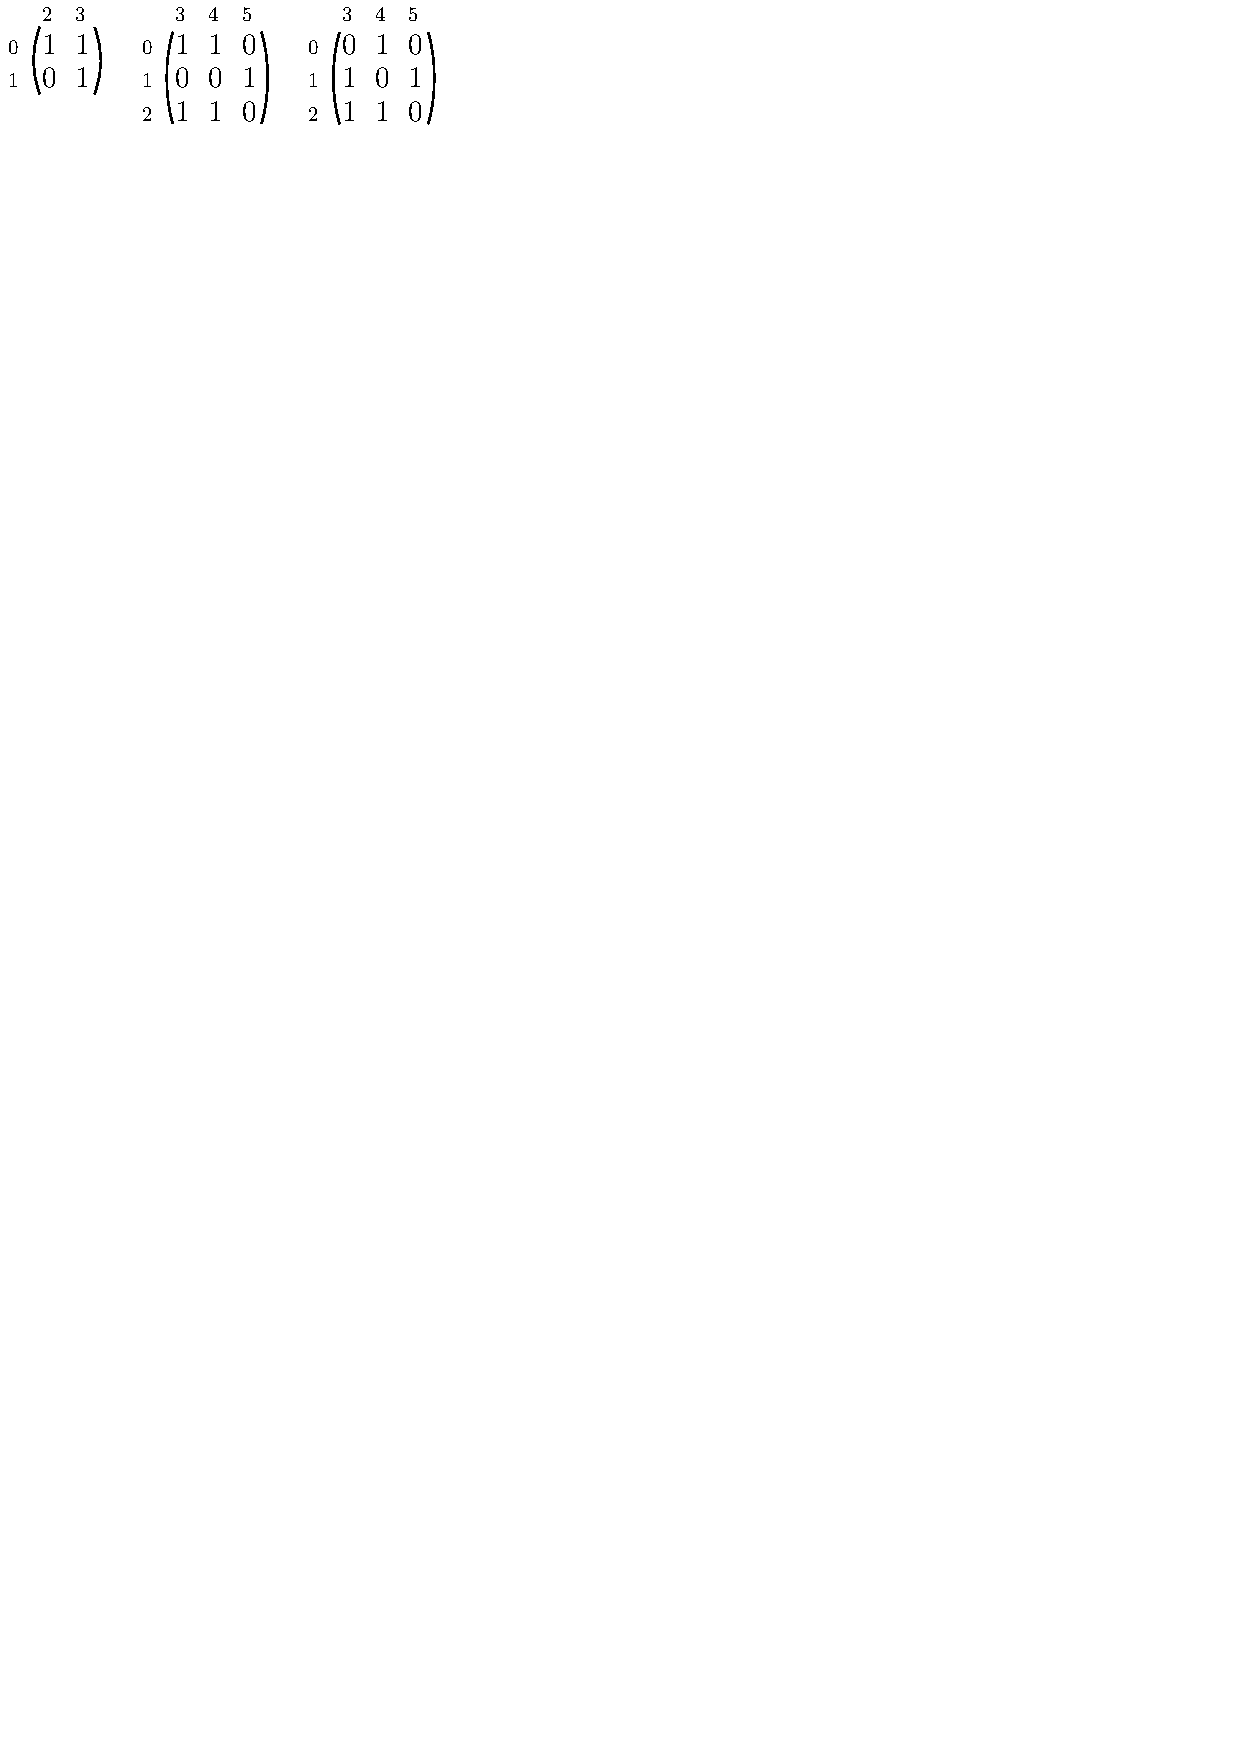
\includegraphics[width=100mm]{../img/avoiding.pdf}
\caption{Matrix $M_1$ contains the pattern $P$, because a mapping $\{(0,0),(1,2),(2,3),(3,4)\}$ satisfies all the conditions. On the other hand, matrix $M_2$ avoids $P$ as there is no such mapping.}
\label{avoiding}
\end{figure}
%\centerline{\mbox{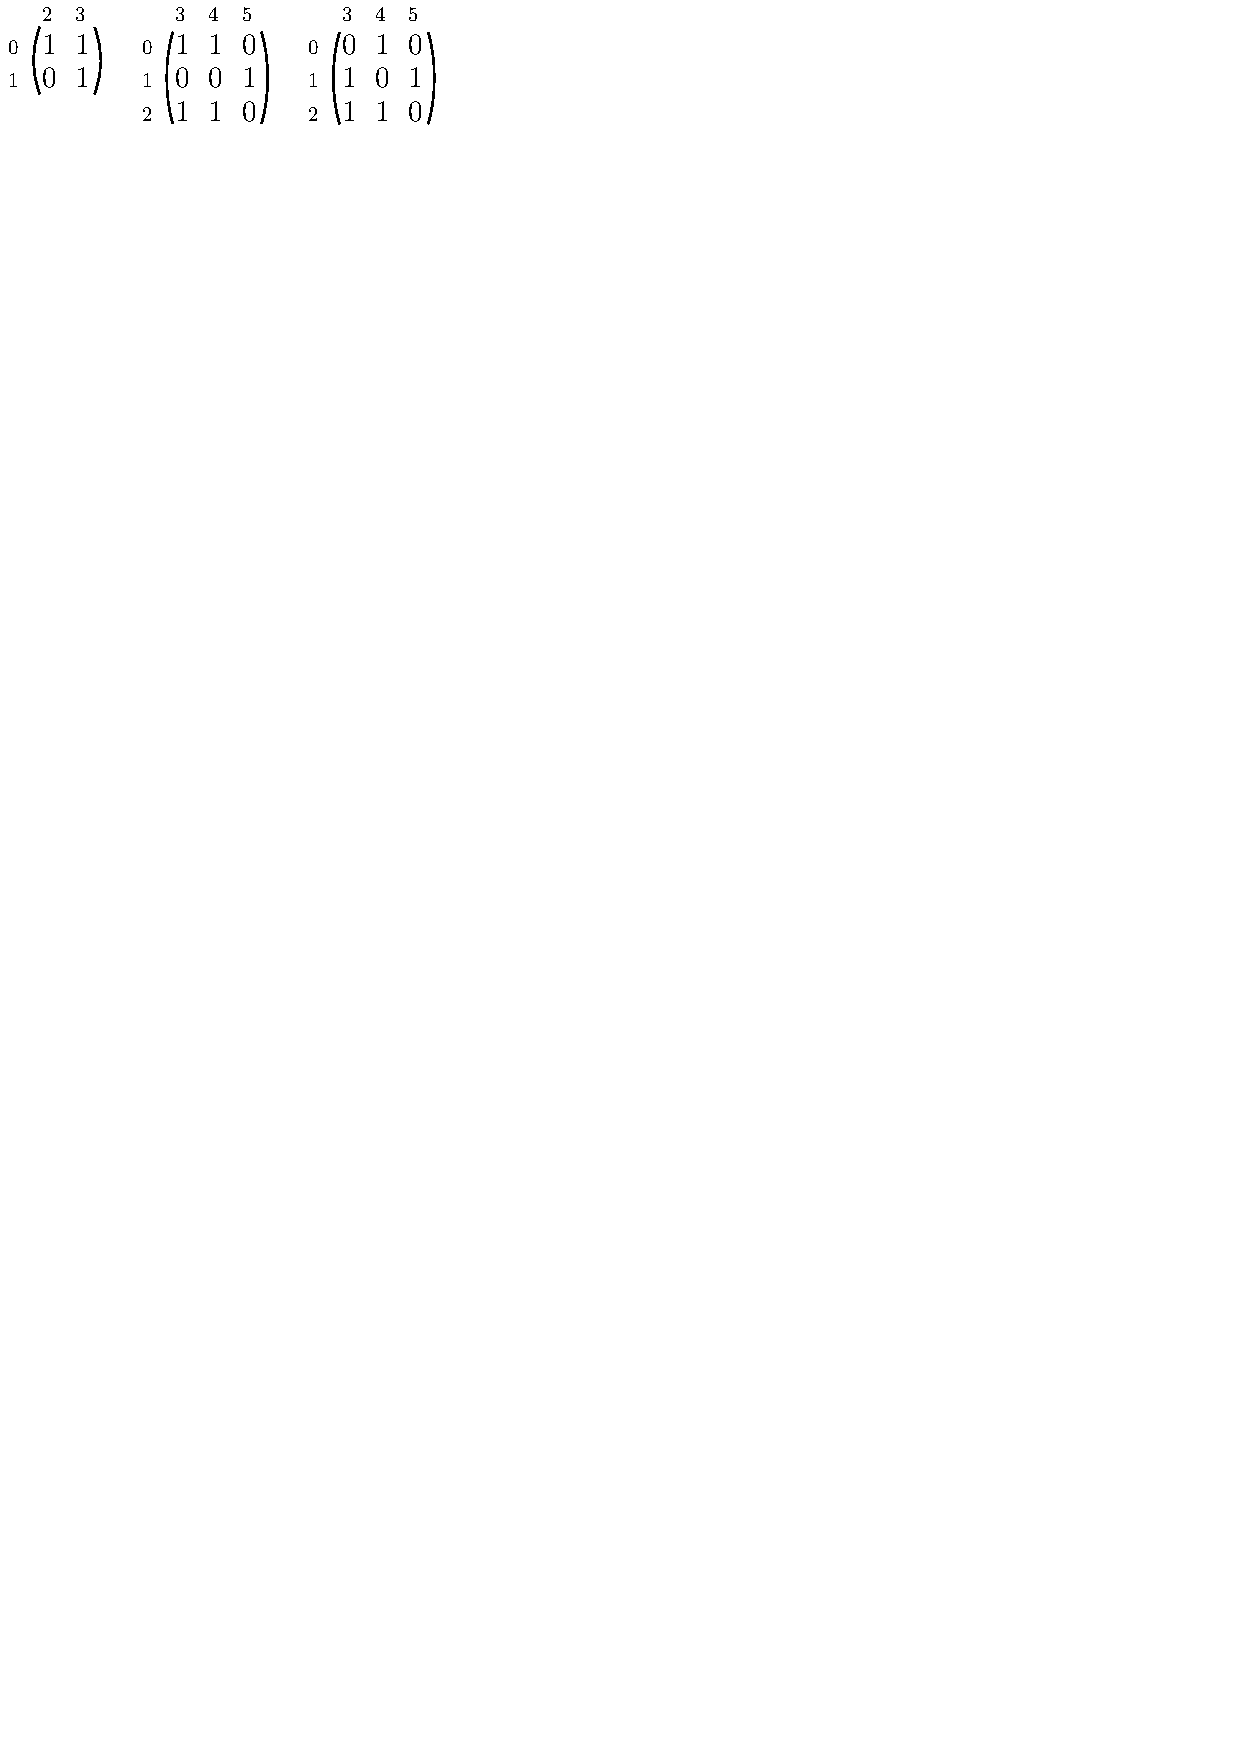
\includegraphics[width=100mm]{../img/avoiding.pdf}}}

The interesting cases are square matrices of size $n$ by $n$, where $n$ is big (going to infinity) and the size of a pattern (not necessarily square matrix) is small (constant). Even for a constant size forbidden pattern it is hard to determine the number of matrices of size $n$ that avoid it or to characterize, what properties they have. Sometimes we consider matrices avoiding more than just one forbidden pattern, in which case we denote the set of all forbidden matrices by $\mathcal{P}$. When a matrix avoids $\mathcal{P}$, it avoids every $P\in\mathcal{P}$. 
\begin{defn}
We denote by $\mathcal{M}_n(\mathcal{P})$ a set of all binary matrices of size $n$ by $n$ avoiding $\mathcal{P}$ as submatrices. We always denote $M$ the square binary matrix for which we test the containing and by $P$ the pattern (if there is one) that is being tested. Moreover, we denote $h$ the height (the number of rows) of $P$ and $w$ its width.
\end{defn}
The area of pattern avoidance has been heavily studied for permutations and it also becomes more popular for their generalization - binary matrices. In most of the areas in combinatorics it is useful to explore properties of random objects and a lot of attention is directed towards random matrices when considering pattern avoidance. The goal of the work is, for given $n\in\mathbb{N}$ and set of forbidden patterns $\mathcal{P}$, to generate a uniformly random $M\in_R\mathcal{M}_n(\mathcal{P})$.
\subsection*{Generating random matrix}
One way to get $M\in_R\mathcal{M}_n(\mathcal{P})$ is to choose a matrix of required size completely at random, for such, test whether it avoids the pattern and simply repeat the process until we find one, which does. However, in the most interesting cases, only a small fraction of all matrices avoid the pattern and the process takes too long, to be practically useful.

For generating random permutations avoiding forbidden pattern, a different technique was introduced in \cite{MadrasLiu}. It uses a randomized process called Markov chain Monte Carlo, which we will abbreviate by MCMC. It is an iterative process, which for a well chosen Markov chain (more in \autoref{chap:mcmc}) approximates a random object. The algorithm by Madras and Liu was developed for permutations (permutation matrices) and it cannot be used for general matrices. In \autoref{sect:mmcmc} we show how to adapt the algorithm, which will lead us to a MCMC algorithm that approximates $M\in_R\mathcal{M}_n(\mathcal{P})$. To produce a good approximation the process needs to do a lot of iterations and despite the fact it is unknown what is the mixing time (the number of iterations required) of a MCMC process, in practice, the method does better than the trivial algorithm.
\subsection*{Testing avoidance}
In each step of our MCMC process we need to test whether a matrix avoids a pattern. We will show a very fast algorithm that only works for a special class of binary matrices (explained in \autoref{chap:walking}) together with a slightly less performing algorithm for a general pattern, which, again, comes as a generalization of an algorithm for permutations from the article by Madras and Liu and is described in \autoref{chap:general}.

In \autoref{chap:imp} we improve both our algorithms and introduce a parallel version of MCMC process, which further increases the performance of matrix generating.

In \autoref{chap:tdoc} some technical details are explained to make reading the code easier for reader and to describe user interface. The last chapter (\autoref{chap:udoc}) contains user documentation.
\addcontentsline{toc}{chapter}{Introduction}

